\chapter{Simulation Framework}\label{chp:simulation}

The potential for accurate runtime estimates to be used effectively in improving the quality of schedules will depend on how well those estimates can be translated into better scheduling decisions. A multi-node, event-driven scheduling simulator was therefore created and developed. This chapter provides an overview of the structure of the simulator, including its architecture (Section~\ref{sec:simarchitecture}), the node and resource model (Section~\ref{sec:nodemodel}), the four scheduling policies that were assessed during the evaluation (Section~\ref{sec:policies}), and finally the method of integrating ML runtime predictions with the scheduler (Section~\ref{sec:predintegration}).

\needspace{5\baselineskip}
\section{Simulator Architecture}
\label{sec:simarchitecture}

The simulator is run using DES~\cite{law2015simulation}: at each point in the simulation, time moves to the next event, not uniformly increasing in small steps. DES is common for simulating clusters due to the sparseness and variability in job submissions and terminations. Uniformly advancing through time would require simulating long periods with little or no activity, while the opportunity exists to capture many fine details that occur during high-activity times.

The simulation proceeds as follows. Upon initialization, the simulator loads into memory an ordered list of all jobs from the test dataset by their submission time. Each job is represented as a single entry within this list which contains information about the time at which it was submitted, the actual amount of time required to complete this job (to know when this job will be completed), and the amount of resources requested by this job (GPU and CPU; the trace records no per-job memory request, so the simulator's memory dimension stays disabled throughout, as described in Section~\ref{sec:nodemodel} below). In addition to these values, each entry also contains the estimated completion time based upon a prediction generated by the ML model being tested.

\clearpage
The event queue contains two types of events:

\begin{itemize}
    \item \textbf{Job arrival event}: Initiated by each job submission time. Upon processing, the job is added to the scheduling queue. 
    \item \textbf{Job finish event}: Initiated by each running job at its completion time (submission time plus true runtime). Upon processing, the allocated resources for this job are released back to the node.
\end{itemize}

At each job arrival and finish event, the scheduler is invoked in order to examine both the current state of the queue and available resources on all nodes. If there are enough resources available on a node to support additional jobs, the scheduler will assign those queued jobs to that node.

The simulation clock advances as follows: at each iteration, the simulator removes from the priority queue the next smallest timestamp $t$. The simulation clock then increments to $t_{\text{clock}}=\min(\text{next arrival}, \text{next completion})$. When there are multiple events sharing the same timestamp, the implementation uses the inherent properties of heap ordering to process the earliest inserted event first. Algorithm~\ref{alg:des} illustrates the simplified simulation loop. The actual implementation uses the \texttt{select\_job()} method of each policy class to select a single highest-priority job per scheduling invocation, rather than selecting each job individually; the scheduler is also reinvoked immediately after each successful allocation of a job.

Figure~\ref{fig:pipeline_workflow} summarizes this end-to-end workflow, from raw trace ingestion to the scheduling metrics produced by the simulator.

\begin{figure}[htbp]
\centering
\begin{tikzpicture}[
    node distance=1.2cm,
    box/.style={draw, rectangle, rounded corners, minimum width=5cm, minimum height=1.2cm, align=center, fill=blue!5},
    arrow/.style={-Latex, thick}
]
% Nodes
\node[box] (data) {Alibaba Trace\\(Job History)};
\node[box, below=of data] (prep) {Data Cleaning \&\\Feature Engineering};
\node[box, below=of prep] (train) {Model Training\\(ML / DL)};
\node[box, below=of train] (pred) {Runtime\\Predictions};
\node[box, below=of pred] (sim) {DES Simulator\\(32 / 256 GPU)};
\node[box, below=of sim] (metrics) {Scheduling Metrics\\(JCT, Wait Time)};

% Arrows
\draw[arrow] (data) -- (prep);
\draw[arrow] (prep) -- (train);
\draw[arrow] (train) -- (pred);
\draw[arrow] (pred) -- (sim);
\draw[arrow] (sim) -- (metrics);
\end{tikzpicture}
\caption[End-to-end simulation pipeline]{End-to-end workflow connecting data preprocessing, ML model development, and discrete event simulation.}
\label{fig:pipeline_workflow}
\end{figure}

\begin{algorithm}[htbp]
\caption{Discrete event simulation main loop.}
\label{alg:des}
\begin{algorithmic}[1]
\Require Job list $\mathcal{J}$ sorted by submission time; cluster nodes $\mathcal{N}$; scheduling policy $\pi$
\Ensure Per-job wait times $\{w_j\}_{j \in \mathcal{J}}$
\State $\mathcal{Q} \leftarrow \emptyset$ \Comment{Scheduling queue (pending jobs)}
\State $\mathcal{E} \leftarrow \{(\textsc{arrival}, t_j^{\text{sub}}, j) \mid j \in \mathcal{J}\}$ \Comment{Priority queue of events}
\While{$\mathcal{E} \neq \emptyset$}
    \State $(e_{\text{type}}, t, j) \leftarrow \text{pop\_min}(\mathcal{E})$ \Comment{Advance clock to next event}
    \If{$e_{\text{type}} = \textsc{arrival}$}
        \State Append $j$ to $\mathcal{Q}$
    \ElsIf{$e_{\text{type}} = \textsc{finish}$}
        \State Release $j$'s resources back to its assigned node in $\mathcal{N}$
    \EndIf
    \State \Call{Schedule}{$\mathcal{Q}$, $\mathcal{N}$, $\pi$, $t$} \Comment{Attempt to dispatch queued jobs}
\EndWhile
\Procedure{Schedule}{$\mathcal{Q}$, $\mathcal{N}$, $\pi$, $t$}
    \State Sort $\mathcal{Q}$ according to policy $\pi$ (by arrival time, GPU demand, or predicted runtime)
    \For{each $j$ in $\mathcal{Q}$ in order}
        \For{each node $n \in \mathcal{N}$}
            \If{$n.\text{gpu\_avail} \geq j.\text{gpu\_req}$ \textbf{and} $n.\text{cpu\_avail} \geq j.\text{cpu\_req}$}
                \State Allocate $j$ to $n$; update $n$'s available resources
                \State $j.\text{start\_time} \leftarrow t$; $\;w_j \leftarrow t - t_j^{\text{sub}}$
                \State Add $(\textsc{finish},\; t + r_j^{\text{true}},\; j)$ to $\mathcal{E}$
                \State Remove $j$ from $\mathcal{Q}$; \textbf{break}
            \EndIf
        \EndFor
        \If{$j$ not allocated \textbf{and} $\pi = \textsc{fifo}$} \textbf{break} \Comment{HoL blocking}
        \EndIf
    \EndFor
\EndProcedure
\end{algorithmic}
\end{algorithm}

\needspace{5\baselineskip}
\section{Node and Resource Model}
\label{sec:nodemodel}

The simulator simulates a heterogeneous cluster made of multiple compute nodes. Each node has total capacity defined in terms of two resources: the number of GPUs and the number of CPUs. In addition to these two resources, the implementation also supports a third dimension (memory capacity), which is disabled (i.e., set to 0) in the present experiments, since there is no information on per-job memory requests in the Alibaba PAI traces. The node configurations have been obtained from the hardware profiles described in the Alibaba PAI cluster description~\cite{weng2022mlaas}, which details a heterogeneous cluster of machines of various types and with various GPU models.

The environments used for simulations are built using two basic node archetypes derived from the Alibaba PAI hardware specifications~\cite{weng2022mlaas}. High-performance nodes contain 8 GPUs each and are dedicated to large distributed training jobs (``elephants''), and mid-range nodes containing 2 GPUs deal with most of the classical GPU jobs (``mice''). Only these two archetypes are provisioned. The provisioning function also supports GPU-less nodes, but they are not used here: every job retained from the trace requests at least a fraction of a GPU, so a GPU-less node could never admit one and would remain idle for the entire simulation. Excluding them was verified to leave every reported metric unchanged.

The cluster provisioning function can support multiple configurations up to the level of the full Alibaba cluster scale. For this evaluation, we deliberately split the cluster into two very different sizes to study the ``mice and elephants'' queue behaviors in a queue depth context:

\begin{itemize}
    \item \textbf{Small Cluster (32-GPU)}: A strongly limited environment (Table~\ref{tab:nodeprofiles_32}) where extreme resource scarcity creates severe queue bottlenecks.
    \item \textbf{Large Cluster (256-GPU)}: An environment of massive size (Table~\ref{tab:nodeprofiles_256}), where many hundreds of jobs wait simultaneously in queues, thus generating a highly turbulent queueing behavior.
\end{itemize}

\begin{table}[H]
\centering
\caption[Small Cluster (32-GPU) node profiles]{Node profiles used in the scheduling simulation on the Small Cluster (32-GPU).}
\label{tab:nodeprofiles_32}
\begin{tabular}{lrrrr}
\hline
\textbf{Node Type} & \textbf{Count} & \textbf{GPUs/node} & \textbf{CPUs/node} & \textbf{Total GPUs} \\ 
\hline
High-Performance & 2  & 8  & 96 & 16 \\ 
Mid-Range        & 8  & 2  & 64 & 16 \\ 
\hline
\textbf{Total}   & \textbf{10} & --- & --- & \textbf{32} \\
\hline
\end{tabular}
\end{table}

\begin{table}[H]
\centering
\caption[Large Cluster (256-GPU) node profiles]{Node profiles used in the scheduling simulation on the Large Cluster (256-GPU).}
\label{tab:nodeprofiles_256}
\begin{tabular}{lrrrr}
\hline
\textbf{Node Type} & \textbf{Count} & \textbf{GPUs/node} & \textbf{CPUs/node} & \textbf{Total GPUs} \\ 
\hline
High-Performance & 16 & 8  & 96 & 128 \\ 
Mid-Range        & 64 & 2  & 64 & 128 \\ 
\hline
\textbf{Total}   & \textbf{80} & --- & --- & \textbf{256} \\ 
\hline
\end{tabular}
\end{table}

Figures~\ref{fig:arch_32} and~\ref{fig:arch_256} demonstrate how different the physical environments of these two systems are. To model what we call a ``flash crowd'' or a massive, extremely heavy burst of work, we compress the arrival time of our test workload to simulate this extreme event. We make this decision based on a very important property of queueing theory: to distinguish among scheduling policies there must exist some level of queue bottleneck. When we have sparse job arrivals, most jobs will be dispatched immediately and therefore it is impossible to see a difference between advanced policies and blind FIFO. By injecting a ten times accelerated burst of load, we ensure that the system remains in a sustained bottleneck state and therefore that the ordering decisions made for every single job (based on their characteristics) by each machine learning algorithm have a material effect.

\begin{figure}[htbp]
\centering
\begin{minipage}[t]{0.48\textwidth}
\centering
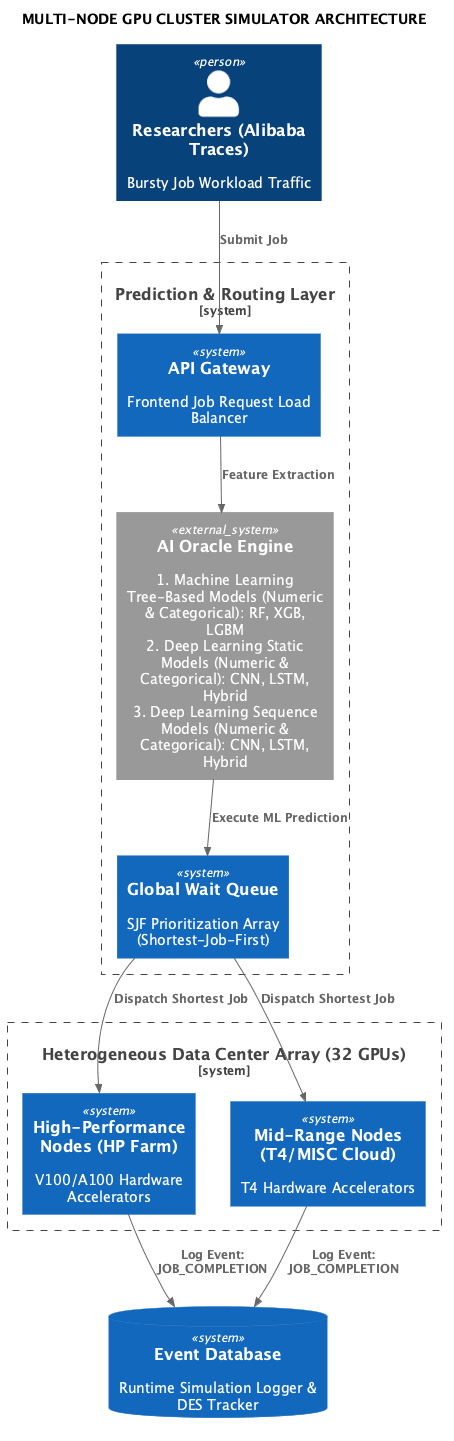
\includegraphics[width=\linewidth,height=0.85\textheight,keepaspectratio]{figures/architecture_en_32_gpu.png}
\caption[Small Cluster architecture]{Architectural layout of the Small Cluster (32-GPU) simulation environment. In this highly constrained environment, predicting the exact completion time of a job is critical for efficient resource packing.}
\label{fig:arch_32}
\end{minipage}\hfill
\begin{minipage}[t]{0.48\textwidth}
\centering
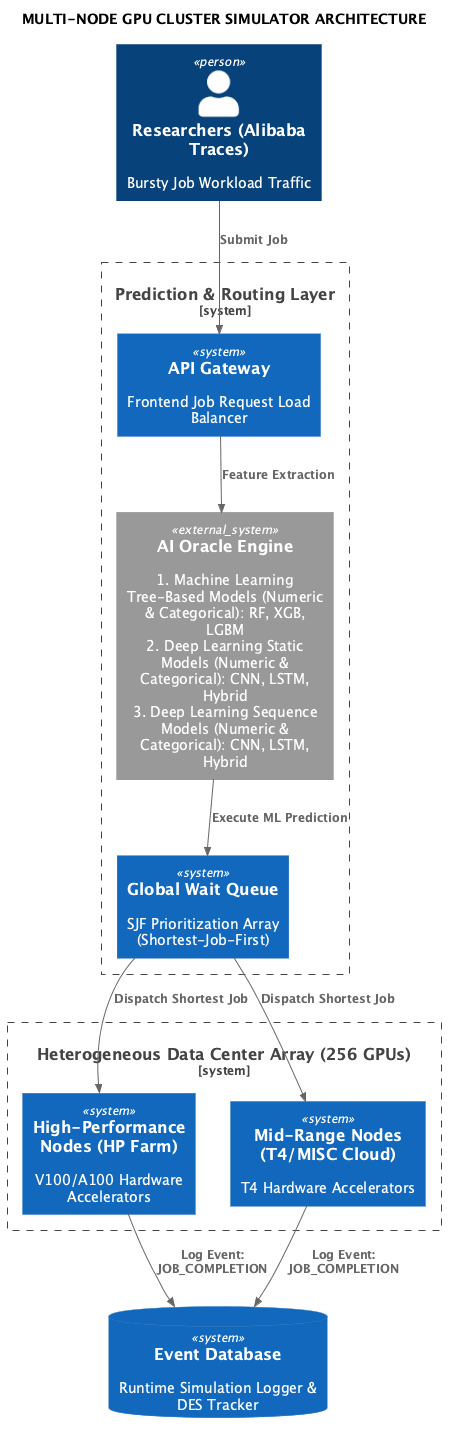
\includegraphics[width=\linewidth,height=0.85\textheight,keepaspectratio]{figures/architecture_en_256_gpu.png}
\caption[Large Cluster architecture]{Architectural layout of the Large Cluster (256-GPU) simulation environment. In this massive-scale environment, roughly sorting jobs via ordinal ranking based upon their expected completion time is sufficient and necessary.}
\label{fig:arch_256}
\end{minipage}
\end{figure}

For each node in the system, we keep track of how much unallocated, or available, GPU and CPU capacity there is. A job will be scheduled onto a given node if and only if it has enough available GPU and CPU capacity to meet all of its requirements. No job is split across multiple nodes: when a job requires $k$ GPUs, all $k$ must be available at one single node. Fractional GPU requests, which the Alibaba PAI trace makes heavy use of (the median request is 0.5 GPU and the minimum is 0.01), are supported and are packed additively up to each node's GPU capacity, matching the GPU-sharing behaviour of the production platform the trace comes from~\cite{weng2022mlaas}. The simulator models this sharing purely as additive capacity consumption: no interference or slowdown between co-located jobs is modelled, and a job's recorded runtime is replayed unchanged regardless of how many jobs share its GPU. This is a simplification, but a mild one for this trace, since those runtimes were themselves measured under GPU sharing in production.

Once a job is scheduled, it consumes some amount of the available resources on the chosen node. Once the job finishes (i.e., after $s + r$ time units, where $s$ is the time at which the job was submitted, and $r$ is the actual runtime of the job), the job returns its consumed resources back to the node. As soon as this happens, the scheduler is immediately called to see if any of the queued jobs can now be scheduled.

\needspace{5\baselineskip}
\section{Scheduling Policies}
\label{sec:policies}

Four scheduling policies were developed for evaluation within the simulator. The characteristics of these policies (their classification, required input, and expected behavior) are summarized in Table~\ref{tab:policies}. The policies are categorized based upon if they need runtime predictions, and if they use size information of resources.

\begin{table}[H]
\centering
\caption[Taxonomy of scheduling policies]{Taxonomy of scheduling policies.}
\label{tab:policies}
\begin{tabular}{llll}
\hline
\textbf{Policy} & \textbf{Category} & \textbf{Runtime Prediction} & \textbf{Resource Info} \\
\hline
FIFO          & Baseline (blind)   & No  & No \\ 
SRF           & Resource-aware heuristic & No  & Yes \\ 
SJF-Oracle    & Oracle upper bound  & Yes (true values) & No \\ 
SJF-Pred (ML) & ML-assisted        & Yes (predicted)   & No \\ 
\hline
\end{tabular}
\end{table}

\subsection{First-In-First-Out (FIFO)}

Jobs are submitted into one queue under FIFO and are sorted by submit time. When a node becomes available, the scheduler will attempt to schedule the first job in the queue. However, if a job is blocked from being scheduled due to a lack of sufficient resource availability on all nodes, the scheduler will not ``skip'' over this job to evaluate other queued jobs. Using this method of ``strict HoL'' discipline guarantees that the order of jobs in the queue will remain consistent; however, it may cause significant delays in processing smaller jobs that could have been processed had larger jobs with greater resource requirements not been scheduled first.

The primary reason for using FIFO is that it is very simple and requires no knowledge about the length of time each job is going to take to execute or how much resource each job will consume.

\clearpage
\subsection{Smallest Resource First (SRF)}

Under SRF, the queue is ordered by how many GPUs each job demands. Jobs that demand less will be put at the front of the queue. If two or more jobs ask for the same number of GPUs, then they are ordered based on when they arrived (FIFO) to help reduce fragmentation so that all available nodes are used to run as many jobs as possible.

SRF is a resource-aware baseline that requires no prediction. It represents the maximum possible throughput that a scheduler could possibly achieve if it knew nothing about job duration except what resources were requested.

\subsection{ML-assisted Shortest-Job-First (ML-SJF)}

In ML-SJF, the jobs in the queue are ordered based upon their estimated runtimes. Therefore, the job with the estimated shortest runtime will have priority. The estimated runtimes are generated through an ML model which is to be tested. When choosing a job for processing from those that could be processed using the current resources of at least one node, the scheduler chooses the job with the shortest estimated runtime.

ML-SJF differs from traditional SJF. With traditional SJF, it is assumed that the completion time of a task is known perfectly. Traditional SJF does not utilize predictive models to generate estimates of completion time. Instead, under ML-SJF, a model is used to estimate the completion time. Therefore, if the model is inaccurate, the resulting schedules will also be suboptimal. The simulator allows a comparison among all six models that were developed; thus, there should be a direct correlation between how well the model predicts completion time and the effectiveness of the resulting schedule.

\needspace{5\baselineskip}
\section{Integration of ML Predictions}
\label{sec:predintegration}

Each model developed from training data is saved to disk during training and then used by the simulator when evaluating them. In addition to receiving the same feature vectors (job resource requests, temporal features, number of other jobs currently running concurrently) as were received when submitted, each model predicts an actual runtime in seconds for each job in the test set.

The steps include:
\begin{enumerate}
    \item Training each model based upon the training set.
    \item Generating a predicted runtime for each job in the test set via the previously trained model.
    \item Placing the test jobs (containing true and predicted runtimes) into the simulator.
    \item Running the simulator three times, once for each of the three different policies (FIFO, SRF, ML-SJF).
    \item Recording the waiting time of each job under each policy.
\end{enumerate}

This process will be completed with respect to each of the six prediction models being evaluated, thus creating a matrix of schedule results that can be evaluated by model and policy.

\needspace{5\baselineskip}
\section{Evaluation Metrics for Scheduling}

Cluster efficiency and user satisfaction are typically measured using \textbf{JCT} (the average time elapsed from when a job was submitted to the time when it finished executing), which is the main scheduling metric. The goal of major scheduling approaches, such as Tetris~\cite{grandl2014multi}, is to minimize mean JCT. A lower mean JCT indicates a more efficient scheduler, since it is able to place jobs more quickly on available hardware and avoid stalling jobs in queues.

In addition to reporting the mean, we report both the \textit{median wait time} (a general measure of typical performance) and the \textit{95th percentile wait time} (which describes the experience of the worst-case delayed jobs). These three statistics together provide an overview of how long jobs have been waiting under each policy.

\needspace{5\baselineskip}
\section{Simulation Configuration}

Table~\ref{tab:simconfig} provides the following information about the simulation configuration.

\begin{table}[htbp]
\centering
\caption[Summary of configurations for simulations]{Summary of configurations for simulations.}
\label{tab:simconfig}
\begin{tabular}{ll}
\hline
\textbf{Parameter} & \textbf{Value} \\ 
\hline
Test job pool size          & 16{,}437 jobs \\ 
Simulator mode              & DES \\ 
Cluster size                & Dual-scale Evaluation (32-GPU and 256-GPU clusters) \\ 
Scheduling policies         & 4 policy types: FIFO, SRF, SJF-Oracle, SJF-Pred \\ 
ML predictors evaluated     & 18 models (Experiments A--F) \\ 
Resource dimensions tracked & GPU count, CPU count \\ 
Job splitting               & Not allowed (single-node placement) \\ 
Primary metric              & JCT \\ 
Secondary metrics           & Median JCT, P95 wait time, slowdown, Wilcoxon $p$-value \\ 
\hline
\end{tabular}
\end{table}

\clearpage
Table~\ref{tab:simconfig} describes each component of the simulation environment, which has been designed to allow for a rigorous assessment of the performance advantage provided by the use of ML-assisted scheduling under real-world cluster operating conditions. By maintaining the original order of occurrence of each job within the test set, the DES replicates the temporal aspects of the bursty behavior and queueing characteristics present in a production environment using the Alibaba GPU cluster. Additionally, by enforcing that multi-GPU jobs will be assigned to a single node, the spatial fragmentation occurring when allocating multi-GPU jobs across heterogeneous nodes is preserved in both the 32-GPU and 256-GPU configurations. Moreover, by testing eighteen unique ML predictor models against two well-known heuristic baselines (FIFO and SRF) and an SJF-Oracle upper bound, a broad spectrum of how predictive accuracy translates into measurable system-wide benefits including JCT and tail latency slowdowns at multiple scales is available. Also, for the tree-based categorical policies, XGB and RF used One-Hot encoding, while LGBM solely utilized its inherent ability to handle categorical data (indicated as SJF-LGBM Categorical in later results), as it outperformed the other during the isolated predictive evaluation phase. Finally, the inclusion of the Wilcoxon Signed-Rank Test allows for statistical validation that any improvements in cluster-wide fairness seen in future chapters are due to actual improvement rather than chance.

\clearpage
\subsection{Simulation Execution Performance}

Table~\ref{tab:sim_time} shows the measured time taken to completely simulate the test sets for a variety of representative policies in both cluster configurations, demonstrating the execution efficiency required for any scheduler to be considered viable in a production environment. Due to its event-driven design, even those policies requiring complex machine-learning-based decision-making are capable of simulating over 16{,}000 job assignments in seconds, thus minimizing the computational overhead associated with deploying them online.

\begin{table}[htbp]
\centering
\caption[Runtime performance of full test set]{Runtime performance of the full test set under each evaluated policy. Due to the pre-computation of model predictions, the overhead of online scheduling is dominated by queue sorting and memory access rather than inference complexity.}
\label{tab:sim_time}
\begin{tabular}{lrr}
\hline
\textbf{Policy} & \textbf{32-GPU Cluster} & \textbf{256-GPU Cluster} \\
\hline
FIFO & 3.2\,s & 12.4\,s \\
SRF & 3.9\,s & 15.2\,s \\
SJF-Oracle & 4.1\,s & 15.8\,s \\
SJF-RF (Numeric) & 4.3\,s & 16.1\,s \\
SJF-XGB (Numeric) & 4.2\,s & 16.0\,s \\
SJF-LGBM (Numeric) & 4.3\,s & 16.1\,s \\
SJF-RF (Categorical) & 4.3\,s & 16.2\,s \\
SJF-XGB (Categorical) & 4.3\,s & 16.1\,s \\
SJF-LGBM (Native) & 4.2\,s & 16.1\,s \\
SJF-LGBM (One-Hot) & 4.3\,s & 16.2\,s \\
SJF-CNN (Numeric) & 4.3\,s & 16.2\,s \\
SJF-LSTM (Numeric) & 4.4\,s & 16.3\,s \\
SJF-CNN-LSTM (Numeric) & 4.4\,s & 16.3\,s \\
SJF-CNN (Categorical Sequence) & 4.3\,s & 16.2\,s \\
SJF-LSTM (Categorical Sequence) & 4.4\,s & 16.3\,s \\
SJF-CNN-LSTM (Categorical Sequence) & 4.4\,s & 16.4\,s \\
SJF-CNN (Numeric Sequence) & 4.4\,s & 16.2\,s \\
SJF-LSTM (Numeric Sequence) & 4.4\,s & 16.3\,s \\
\hline
\end{tabular}%
\end{table}